\documentclass[twoside]{book}

% Packages required by doxygen
\usepackage{fixltx2e}
\usepackage{calc}
\usepackage{doxygen}
\usepackage[export]{adjustbox} % also loads graphicx
\usepackage{graphicx}
\usepackage[utf8]{inputenc}
\usepackage{makeidx}
\usepackage{multicol}
\usepackage{multirow}
\PassOptionsToPackage{warn}{textcomp}
\usepackage{textcomp}
\usepackage[nointegrals]{wasysym}
\usepackage[table]{xcolor}

% NLS support packages
\usepackage[T2A]{fontenc}
\usepackage[russian]{babel}

% Font selection
\usepackage[T1]{fontenc}
\usepackage[scaled=.90]{helvet}
\usepackage{courier}
\usepackage{amssymb}
\usepackage{sectsty}
\renewcommand{\familydefault}{\sfdefault}
\allsectionsfont{%
  \fontseries{bc}\selectfont%
  \color{darkgray}%
}
\renewcommand{\DoxyLabelFont}{%
  \fontseries{bc}\selectfont%
  \color{darkgray}%
}
\newcommand{\+}{\discretionary{\mbox{\scriptsize$\hookleftarrow$}}{}{}}

% Page & text layout
\usepackage{geometry}
\geometry{%
  a4paper,%
  top=2.5cm,%
  bottom=2.5cm,%
  left=2.5cm,%
  right=2.5cm%
}
\tolerance=750
\hfuzz=15pt
\hbadness=750
\setlength{\emergencystretch}{15pt}
\setlength{\parindent}{0cm}
\setlength{\parskip}{0.2cm}
\makeatletter
\renewcommand{\paragraph}{%
  \@startsection{paragraph}{4}{0ex}{-1.0ex}{1.0ex}{%
    \normalfont\normalsize\bfseries\SS@parafont%
  }%
}
\renewcommand{\subparagraph}{%
  \@startsection{subparagraph}{5}{0ex}{-1.0ex}{1.0ex}{%
    \normalfont\normalsize\bfseries\SS@subparafont%
  }%
}
\makeatother

% Headers & footers
\usepackage{fancyhdr}
\pagestyle{fancyplain}
\fancyhead[LE]{\fancyplain{}{\bfseries\thepage}}
\fancyhead[CE]{\fancyplain{}{}}
\fancyhead[RE]{\fancyplain{}{\bfseries\leftmark}}
\fancyhead[LO]{\fancyplain{}{\bfseries\rightmark}}
\fancyhead[CO]{\fancyplain{}{}}
\fancyhead[RO]{\fancyplain{}{\bfseries\thepage}}
\fancyfoot[LE]{\fancyplain{}{}}
\fancyfoot[CE]{\fancyplain{}{}}
\fancyfoot[RE]{\fancyplain{}{\bfseries\scriptsize Документация по My Project. Последние изменения\+: Сб 26 Дек 2015 20\+:37\+:30. Создано системой Doxygen }}
\fancyfoot[LO]{\fancyplain{}{\bfseries\scriptsize Документация по My Project. Последние изменения\+: Сб 26 Дек 2015 20\+:37\+:30. Создано системой Doxygen }}
\fancyfoot[CO]{\fancyplain{}{}}
\fancyfoot[RO]{\fancyplain{}{}}
\renewcommand{\footrulewidth}{0.4pt}
\renewcommand{\chaptermark}[1]{%
  \markboth{#1}{}%
}
\renewcommand{\sectionmark}[1]{%
  \markright{\thesection\ #1}%
}

% Indices & bibliography
\usepackage{natbib}
\usepackage[titles]{tocloft}
\setcounter{tocdepth}{3}
\setcounter{secnumdepth}{5}
\makeindex

% Hyperlinks (required, but should be loaded last)
\usepackage{ifpdf}
\ifpdf
  \usepackage[pdftex,pagebackref=true]{hyperref}
\else
  \usepackage[ps2pdf,pagebackref=true]{hyperref}
\fi
\hypersetup{%
  colorlinks=true,%
  linkcolor=blue,%
  citecolor=blue,%
  unicode%
}

% Custom commands
\newcommand{\clearemptydoublepage}{%
  \newpage{\pagestyle{empty}\cleardoublepage}%
}


%===== C O N T E N T S =====

\begin{document}

% Titlepage & ToC
\hypersetup{pageanchor=false,
             bookmarks=true,
             bookmarksnumbered=true,
             pdfencoding=unicode
            }
\pagenumbering{roman}
\begin{titlepage}
\vspace*{7cm}
\begin{center}%
{\Large My Project }\\
\vspace*{1cm}
{\large Создано системой Doxygen 1.8.10}\\
\vspace*{0.5cm}
{\small Сб 26 Дек 2015 20:37:30}\\
\end{center}
\end{titlepage}
\clearemptydoublepage
\tableofcontents
\clearemptydoublepage
\pagenumbering{arabic}
\hypersetup{pageanchor=true}

%--- Begin generated contents ---
\chapter{Алфавитный указатель пространств имен}
\section{Пространства имен}
Полный список пространств имен.\begin{DoxyCompactList}
\item\contentsline{section}{\hyperlink{namespace_ui}{Ui} }{\pageref{namespace_ui}}{}
\end{DoxyCompactList}

\chapter{Иерархический список классов}
\section{Иерархия классов}
Иерархия классов.\begin{DoxyCompactList}
\item \contentsline{section}{G\+P\+I\+O\+Pin}{\pageref{struct_g_p_i_o_pin}}{}
\item \contentsline{section}{G\+P\+I\+O\+Struct}{\pageref{struct_g_p_i_o_struct}}{}
\item \contentsline{section}{Opora\+Data\+Struct}{\pageref{struct_opora_data_struct}}{}
\item Q\+Main\+Window\begin{DoxyCompactList}
\item \contentsline{section}{Main\+Window}{\pageref{class_main_window}}{}
\end{DoxyCompactList}
\end{DoxyCompactList}

\chapter{Алфавитный указатель классов}
\section{Классы}
Классы с их кратким описанием.\begin{DoxyCompactList}
\item\contentsline{section}{\hyperlink{struct_g_p_i_o_pin}{G\+P\+I\+O\+Pin} \\*Структура вывода для микроконтроллера Эта структура предназначена для управления выводом микроконтроллера }{\pageref{struct_g_p_i_o_pin}}{}
\item\contentsline{section}{\hyperlink{struct_g_p_i_o_struct}{G\+P\+I\+O\+Struct} \\*Настройка порта Gpio Эта структура предназначена для управления портом микроконтроллера }{\pageref{struct_g_p_i_o_struct}}{}
\item\contentsline{section}{\hyperlink{class_main_window}{Main\+Window} }{\pageref{class_main_window}}{}
\item\contentsline{section}{\hyperlink{struct_opora_data_struct}{Opora\+Data\+Struct} \\*Настройка опоры Эта структура предназначена для настройки опоры микроконтроллера 1986\+V\+E1\+T }{\pageref{struct_opora_data_struct}}{}
\end{DoxyCompactList}

\chapter{Список файлов}
\section{Файлы}
Полный список файлов.\begin{DoxyCompactList}
\item\contentsline{section}{\hyperlink{main_8cpp}{main.\+cpp} }{\pageref{main_8cpp}}{}
\item\contentsline{section}{\hyperlink{mainwindow_8cpp}{mainwindow.\+cpp} }{\pageref{mainwindow_8cpp}}{}
\item\contentsline{section}{\hyperlink{mainwindow_8h}{mainwindow.\+h} }{\pageref{mainwindow_8h}}{}
\item\contentsline{section}{\hyperlink{struct__code_8h}{struct\+\_\+code.\+h} \\*Файл данных для генератора кода }{\pageref{struct__code_8h}}{}
\end{DoxyCompactList}

\chapter{Пространства имен}
\hypertarget{namespace_ui}{}\section{Пространство имен Ui}
\label{namespace_ui}\index{Ui@{Ui}}

\chapter{Классы}
\hypertarget{struct_g_p_i_o_pin}{}\section{Структура G\+P\+I\+O\+Pin}
\label{struct_g_p_i_o_pin}\index{G\+P\+I\+O\+Pin@{G\+P\+I\+O\+Pin}}


Структура вывода для микроконтроллера Эта структура предназначена для управления выводом микроконтроллера  




{\ttfamily \#include $<$struct\+\_\+code.\+h$>$}

\subsection*{Открытые атрибуты}
\begin{DoxyCompactItemize}
\item 
char \hyperlink{struct_g_p_i_o_pin_a7fb5dbc1ae96fdcf98d3a2aa27383460}{R\+X\+T\+X}
\begin{DoxyCompactList}\small\item\em управление портом \end{DoxyCompactList}\end{DoxyCompactItemize}


\subsection{Подробное описание}
Структура вывода для микроконтроллера Эта структура предназначена для управления выводом микроконтроллера 

См. определение в файле struct\+\_\+code.\+h строка 15



\subsection{Данные класса}
\hypertarget{struct_g_p_i_o_pin_a7fb5dbc1ae96fdcf98d3a2aa27383460}{}\index{G\+P\+I\+O\+Pin@{G\+P\+I\+O\+Pin}!R\+X\+T\+X@{R\+X\+T\+X}}
\index{R\+X\+T\+X@{R\+X\+T\+X}!G\+P\+I\+O\+Pin@{G\+P\+I\+O\+Pin}}
\subsubsection[{R\+X\+T\+X}]{\setlength{\rightskip}{0pt plus 5cm}char G\+P\+I\+O\+Pin\+::\+R\+X\+T\+X}\label{struct_g_p_i_o_pin_a7fb5dbc1ae96fdcf98d3a2aa27383460}


управление портом 



См. определение в файле struct\+\_\+code.\+h строка 17



Объявления и описания членов структуры находятся в файле\+:\begin{DoxyCompactItemize}
\item 
\hyperlink{struct__code_8h}{struct\+\_\+code.\+h}\end{DoxyCompactItemize}

\hypertarget{struct_g_p_i_o_struct}{}\section{Структура G\+P\+I\+O\+Struct}
\label{struct_g_p_i_o_struct}\index{G\+P\+I\+O\+Struct@{G\+P\+I\+O\+Struct}}


Настройка порта Gpio Эта структура предназначена для управления портом микроконтроллера  




{\ttfamily \#include $<$struct\+\_\+code.\+h$>$}

\subsection*{Открытые атрибуты}
\begin{DoxyCompactItemize}
\item 
struct G\+P\+I\+O\+P\+In \hyperlink{struct_g_p_i_o_struct_a86de6755c894e9527145c87cfa387f2c}{Pin} \mbox{[}16\mbox{]}
\begin{DoxyCompactList}\small\item\em вывод микроконтроллера \end{DoxyCompactList}\end{DoxyCompactItemize}


\subsection{Подробное описание}
Настройка порта Gpio Эта структура предназначена для управления портом микроконтроллера 

См. определение в файле struct\+\_\+code.\+h строка 23



\subsection{Данные класса}
\hypertarget{struct_g_p_i_o_struct_a86de6755c894e9527145c87cfa387f2c}{}\index{G\+P\+I\+O\+Struct@{G\+P\+I\+O\+Struct}!Pin@{Pin}}
\index{Pin@{Pin}!G\+P\+I\+O\+Struct@{G\+P\+I\+O\+Struct}}
\subsubsection[{Pin}]{\setlength{\rightskip}{0pt plus 5cm}struct G\+P\+I\+O\+P\+In G\+P\+I\+O\+Struct\+::\+Pin\mbox{[}16\mbox{]}}\label{struct_g_p_i_o_struct_a86de6755c894e9527145c87cfa387f2c}


вывод микроконтроллера 



См. определение в файле struct\+\_\+code.\+h строка 25



Объявления и описания членов структуры находятся в файле\+:\begin{DoxyCompactItemize}
\item 
\hyperlink{struct__code_8h}{struct\+\_\+code.\+h}\end{DoxyCompactItemize}

\hypertarget{class_main_window}{}\section{Класс Main\+Window}
\label{class_main_window}\index{Main\+Window@{Main\+Window}}


{\ttfamily \#include $<$mainwindow.\+h$>$}

Граф наследования\+:Main\+Window\+:\begin{figure}[H]
\begin{center}
\leavevmode
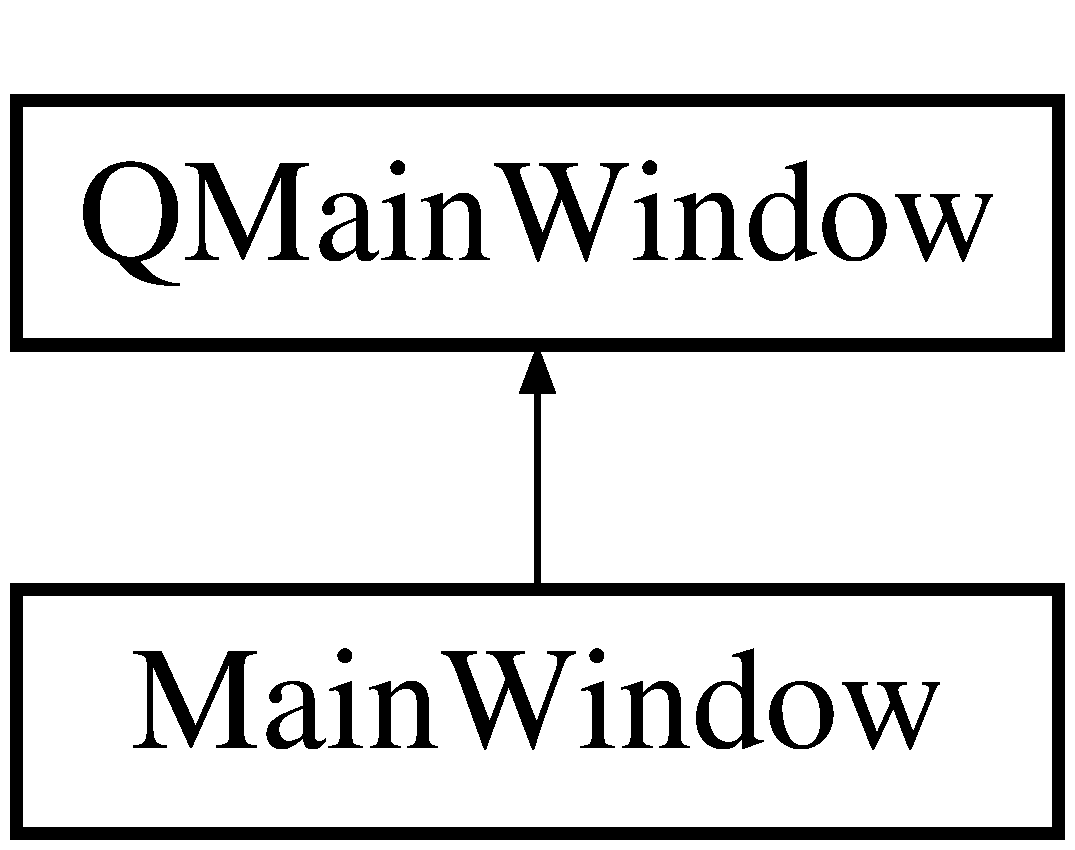
\includegraphics[height=2.000000cm]{class_main_window}
\end{center}
\end{figure}
\subsection*{Открытые члены}
\begin{DoxyCompactItemize}
\item 
\hyperlink{class_main_window_a8b244be8b7b7db1b08de2a2acb9409db}{Main\+Window} (Q\+Widget $\ast$parent=0)
\item 
\hyperlink{class_main_window_ae98d00a93bc118200eeef9f9bba1dba7}{$\sim$\+Main\+Window} ()
\end{DoxyCompactItemize}
\subsection*{Открытые атрибуты}
\begin{DoxyCompactItemize}
\item 
Q\+String \hyperlink{class_main_window_a04a17ff8d2a8277e3d4802fe73707d00}{file}
\end{DoxyCompactItemize}


\subsection{Подробное описание}


См. определение в файле mainwindow.\+h строка 11



\subsection{Конструктор(ы)}
\hypertarget{class_main_window_a8b244be8b7b7db1b08de2a2acb9409db}{}\index{Main\+Window@{Main\+Window}!Main\+Window@{Main\+Window}}
\index{Main\+Window@{Main\+Window}!Main\+Window@{Main\+Window}}
\subsubsection[{Main\+Window(\+Q\+Widget $\ast$parent=0)}]{\setlength{\rightskip}{0pt plus 5cm}Main\+Window\+::\+Main\+Window (
\begin{DoxyParamCaption}
\item[{Q\+Widget $\ast$}]{parent = {\ttfamily 0}}
\end{DoxyParamCaption}
)\hspace{0.3cm}{\ttfamily [explicit]}}\label{class_main_window_a8b244be8b7b7db1b08de2a2acb9409db}


См. определение в файле mainwindow.\+cpp строка 6

\hypertarget{class_main_window_ae98d00a93bc118200eeef9f9bba1dba7}{}\index{Main\+Window@{Main\+Window}!````~Main\+Window@{$\sim$\+Main\+Window}}
\index{````~Main\+Window@{$\sim$\+Main\+Window}!Main\+Window@{Main\+Window}}
\subsubsection[{$\sim$\+Main\+Window()}]{\setlength{\rightskip}{0pt plus 5cm}Main\+Window\+::$\sim$\+Main\+Window (
\begin{DoxyParamCaption}
{}
\end{DoxyParamCaption}
)}\label{class_main_window_ae98d00a93bc118200eeef9f9bba1dba7}


См. определение в файле mainwindow.\+cpp строка 13



\subsection{Данные класса}
\hypertarget{class_main_window_a04a17ff8d2a8277e3d4802fe73707d00}{}\index{Main\+Window@{Main\+Window}!file@{file}}
\index{file@{file}!Main\+Window@{Main\+Window}}
\subsubsection[{file}]{\setlength{\rightskip}{0pt plus 5cm}Q\+String Main\+Window\+::file}\label{class_main_window_a04a17ff8d2a8277e3d4802fe73707d00}


См. определение в файле mainwindow.\+h строка 18



Объявления и описания членов классов находятся в файлах\+:\begin{DoxyCompactItemize}
\item 
\hyperlink{mainwindow_8h}{mainwindow.\+h}\item 
\hyperlink{mainwindow_8cpp}{mainwindow.\+cpp}\end{DoxyCompactItemize}

\hypertarget{struct_opora_data_struct}{}\section{Структура Opora\+Data\+Struct}
\label{struct_opora_data_struct}\index{Opora\+Data\+Struct@{Opora\+Data\+Struct}}


Настройка опоры Эта структура предназначена для настройки опоры микроконтроллера 1986\+V\+E1\+T.  




{\ttfamily \#include $<$struct\+\_\+code.\+h$>$}

\subsection*{Открытые атрибуты}
\begin{DoxyCompactItemize}
\item 
struct \hyperlink{struct_g_p_i_o_struct}{G\+P\+I\+O\+Struct} \hyperlink{struct_opora_data_struct_a390c020a4cec758af905415a634b4722}{G\+P\+I\+O\+Port} \mbox{[}6\mbox{]}
\end{DoxyCompactItemize}


\subsection{Подробное описание}
Настройка опоры Эта структура предназначена для настройки опоры микроконтроллера 1986\+V\+E1\+T. 

См. определение в файле struct\+\_\+code.\+h строка 31



\subsection{Данные класса}
\hypertarget{struct_opora_data_struct_a390c020a4cec758af905415a634b4722}{}\index{Opora\+Data\+Struct@{Opora\+Data\+Struct}!G\+P\+I\+O\+Port@{G\+P\+I\+O\+Port}}
\index{G\+P\+I\+O\+Port@{G\+P\+I\+O\+Port}!Opora\+Data\+Struct@{Opora\+Data\+Struct}}
\subsubsection[{G\+P\+I\+O\+Port}]{\setlength{\rightskip}{0pt plus 5cm}struct {\bf G\+P\+I\+O\+Struct} Opora\+Data\+Struct\+::\+G\+P\+I\+O\+Port\mbox{[}6\mbox{]}}\label{struct_opora_data_struct_a390c020a4cec758af905415a634b4722}


См. определение в файле struct\+\_\+code.\+h строка 33



Объявления и описания членов структуры находятся в файле\+:\begin{DoxyCompactItemize}
\item 
\hyperlink{struct__code_8h}{struct\+\_\+code.\+h}\end{DoxyCompactItemize}

\chapter{Файлы}
\hypertarget{main_8cpp}{}\section{Файл main.\+cpp}
\label{main_8cpp}\index{main.\+cpp@{main.\+cpp}}
{\ttfamily \#include \char`\"{}mainwindow.\+h\char`\"{}}\\*
{\ttfamily \#include $<$Q\+Application$>$}\\*
\subsection*{Функции}
\begin{DoxyCompactItemize}
\item 
int \hyperlink{main_8cpp_a0ddf1224851353fc92bfbff6f499fa97}{main} (int argc, char $\ast$argv\mbox{[}$\,$\mbox{]})
\end{DoxyCompactItemize}


\subsection{Функции}
\hypertarget{main_8cpp_a0ddf1224851353fc92bfbff6f499fa97}{}\index{main.\+cpp@{main.\+cpp}!main@{main}}
\index{main@{main}!main.\+cpp@{main.\+cpp}}
\subsubsection[{main(int argc, char $\ast$argv[])}]{\setlength{\rightskip}{0pt plus 5cm}int main (
\begin{DoxyParamCaption}
\item[{int}]{argc, }
\item[{char $\ast$}]{argv\mbox{[}$\,$\mbox{]}}
\end{DoxyParamCaption}
)}\label{main_8cpp_a0ddf1224851353fc92bfbff6f499fa97}


См. определение в файле main.\+cpp строка 4


\hypertarget{mainwindow_8cpp}{}\section{Файл mainwindow.\+cpp}
\label{mainwindow_8cpp}\index{mainwindow.\+cpp@{mainwindow.\+cpp}}
{\ttfamily \#include \char`\"{}mainwindow.\+h\char`\"{}}\\*
{\ttfamily \#include \char`\"{}ui\+\_\+mainwindow.\+h\char`\"{}}\\*
{\ttfamily \#include \char`\"{}struct\+\_\+code.\+h\char`\"{}}\\*
{\ttfamily \#include $<$qfile.\+h$>$}\\*
{\ttfamily \#include $<$qfiledialog.\+h$>$}\\*

\hypertarget{mainwindow_8h}{}\section{Файл mainwindow.\+h}
\label{mainwindow_8h}\index{mainwindow.\+h@{mainwindow.\+h}}
{\ttfamily \#include $<$Q\+Main\+Window$>$}\\*
{\ttfamily \#include \char`\"{}struct\+\_\+code.\+h\char`\"{}}\\*
\subsection*{Классы}
\begin{DoxyCompactItemize}
\item 
class \hyperlink{class_main_window}{Main\+Window}
\end{DoxyCompactItemize}
\subsection*{Пространства имен}
\begin{DoxyCompactItemize}
\item 
 \hyperlink{namespace_ui}{Ui}
\end{DoxyCompactItemize}

\hypertarget{struct__code_8h}{}\section{Файл struct\+\_\+code.\+h}
\label{struct__code_8h}\index{struct\+\_\+code.\+h@{struct\+\_\+code.\+h}}


Файл данных для генератора кода  


\subsection*{Классы}
\begin{DoxyCompactItemize}
\item 
struct \hyperlink{struct_g_p_i_o_pin}{G\+P\+I\+O\+Pin}
\begin{DoxyCompactList}\small\item\em Структура вывода для микроконтроллера Эта структура предназначена для управления выводом микроконтроллера \end{DoxyCompactList}\item 
struct \hyperlink{struct_g_p_i_o_struct}{G\+P\+I\+O\+Struct}
\begin{DoxyCompactList}\small\item\em Настройка порта Gpio Эта структура предназначена для управления портом микроконтроллера \end{DoxyCompactList}\item 
struct \hyperlink{struct_opora_data_struct}{Opora\+Data\+Struct}
\begin{DoxyCompactList}\small\item\em Настройка опоры Эта структура предназначена для настройки опоры микроконтроллера 1986\+V\+E1\+T. \end{DoxyCompactList}\end{DoxyCompactItemize}


\subsection{Подробное описание}
Файл данных для генератора кода 

\begin{DoxyAuthor}{Автор}
Гусенков.\+С.\+В 
\end{DoxyAuthor}
\begin{DoxyVersion}{Версия}
1.\+0 
\end{DoxyVersion}
\begin{DoxyDate}{Дата}
23 Декабря 2015 года В этом файле находится набор стрктур для генерации кода 
\end{DoxyDate}

%--- End generated contents ---

% Index
\backmatter
\newpage
\phantomsection
\clearemptydoublepage
\addcontentsline{toc}{chapter}{Алфавитный указатель}
\printindex

\end{document}
